\begin{figure}[ht]
    \centering
    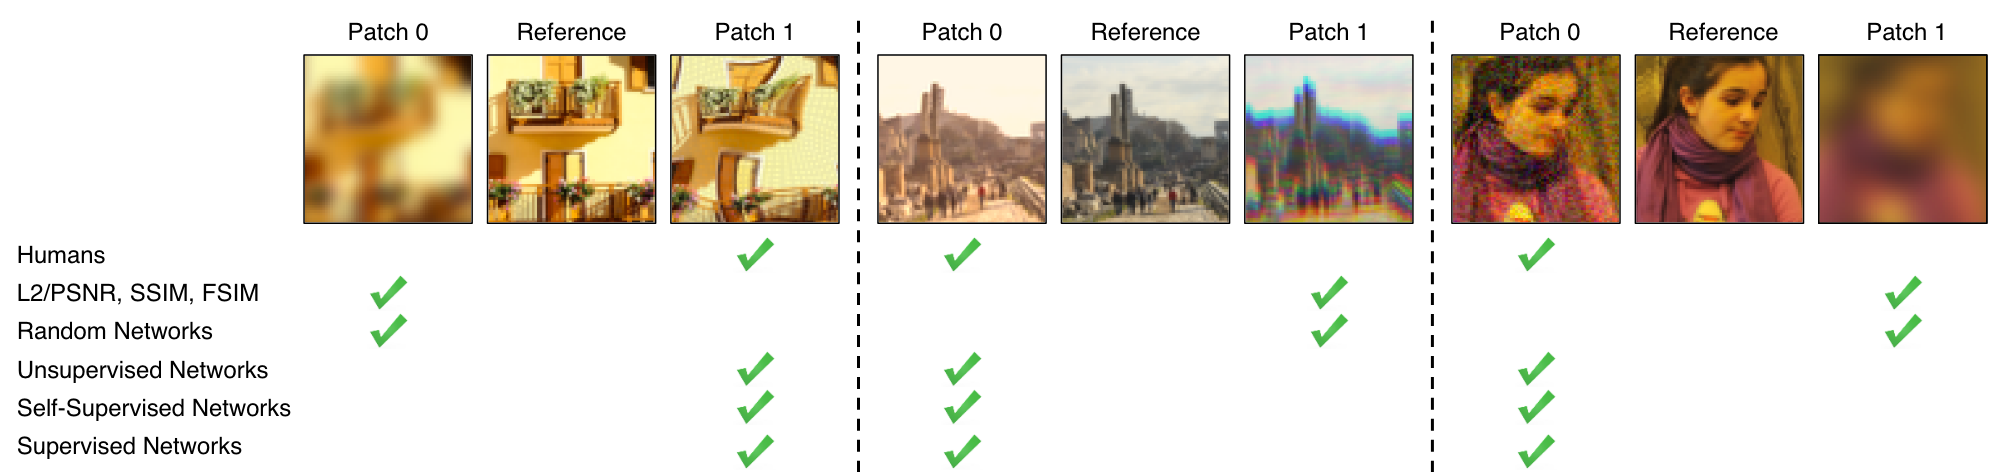
\includegraphics[width=1.0\textwidth]{figures/lpips.png}
    \caption[LPIPS - Learned Perceptual Image Patch Similarity]{\acrshort{lpips} is trained to perceive image similarity the same way humans do. The dataset used to train the similarity metric contains two types of perceptual judgments; \acrshort{2afc} and \acrshort{jnd}. Figure 1 from \acrshort{lpips} \cite{zhang_unreasonable_2018}.}
    \label{fig:lpips}
\end{figure}

